\begin{frame}{\insertsubsection}
  \begin{onlyenv}<1>
    \begin{itemize}
    \item Traits (static and dynamic dispatching)
    \item Zero sized types
    \item Closures
    \item Markers
    \item Higher-kinded types
    \item Compile-time function execution
    \item ...
    \end{itemize}
  \end{onlyenv}

  \begin{onlyenv}<2>%
    \begin{columns}
      \begin{column}{.5\textwidth}
        \begin{itemize}
        \item Python: \mintinline{python}{sum(range(1000))} --- 1000 iterations
          and 1000 additions
        \item Rust: \mintinline{rust}{(0..1000).sum()} --- 499500
        \end{itemize}
      \end{column}
      \begin{column}{.6\textwidth}
        \center%
        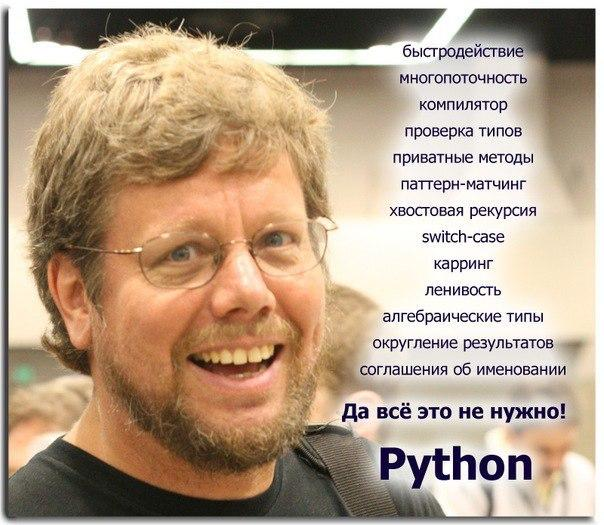
\includegraphics[height = .9\textheight]{python_bad.jpg}%
      \end{column}
    \end{columns}
  \end{onlyenv}

  \note<1>{

    В Rust реализовано \textbf{множество техник}, которые позволяют
    \textbf{избежать накладных расходов при написании высокоуровневого кода}.

    \textbf{С++ также обладает} zero-cost abstractions, т. е. за
    высокоуровневыми абстракциями прячется высокоэффективный код (абстракции без
    накладных расходов). Но даже самые важные C++ люди утверждают, что
    \textbf{им далеко до Rust}, т. к. чтобы достигнуть такого уровня абстракций,
    придётся поломать весь язык и обратную совместимость.

  }

  \note<2>{

    Извините, не мог сдержаться, у меня просто \textbf{полыхает от Python}.

    Самым примитивным примером может послужить вычисление суммы.

  }
\end{frame}
